%%==================================================
%% chapter02.tex for SJTU Master Thesis
%% based on CASthesis
%% modified by wei.jianwen@gmail.com
%% Encoding: UTF-8
%%==================================================

\chapter{研究方法与系统概览}
\label{chap:system}
继第\ref{chap:what}章阐述了本文的研究背景与目的后,本章将进一步介绍本文研究所采用的方法。其中,视频透视技术用于制作混合现实眼镜;
而融合本文所设计的系统多设备间的手势识别技术则用于结合本文所设计的系统所涉及的多种设备输入,使之识别更稳定的手势;最后,针对帮助用户更好地建模而采用沿法向拉伸的自由虚拟网格平面。
此处为基本的技术提要,在第\ref{chap:interaction}章对手势识别有更详细的补充,第\ref{chap:3DModel}章对自由虚拟网格平面的设计有更多的说明。
然后本章将系统划分为多个模块一一介绍,先基本了解本文系统的组成部分,以便进一步深入细节。
\section{研究方法}

\subsection{视频透视技术}
考虑到增强与混合现实应用中经常需要处理的真实物体与虚拟物体间的遮挡,和不同光线下光学透视眼镜受到的影响,本文决定制作一个视频透视\upcite{rolland2000optical}眼镜来完成本文的研究工作。
视频透视技术通过相机拍摄真实场景,利用数字图像处理的方式从图像中获得信息,让佩戴者通过观察数字图像感知真实场景,其中涉及双目相机的标定与图像校正来制作视频透视眼镜,将实际见到的场景经过变化后作为眼镜的输入。
通过得到两个相机的内参与所拍摄的图像进行双目标定与校正,计算其相同点在不同相机中的位置,得到视差,通过视差计算三维坐标数据,因而得到两个相机的外参,而后对两个相机获取到的图片进行校正。

\subsection{融合视觉和LeapMotion的手势识别技术}
考虑到本文工作将采用双目相机和Leap Motion作为输入系统,本文工作决定融合双目相机的输入,与Leap Motion\upcite{motion2012leap}结合,获取更稳定的手势信息。
本文所设计的系统利用OpenCV\upcite{opencv}双目标定对双目相机进行标定,再与LeapMotion标定,从而得到当前场景手的关键点的坐标和色彩信息。
然后对每个设计的手势进行样本采集,分别训练每个手势。
结合LeapMotion得到的手的关键节点信息,当手的节点坐标与手的形状同时满足所设计的手势要求,则识别成功。
为了增加手势识别的稳定性,每个手势的识别会考虑邻近帧的情况,将邻近帧中被成功识别的手势作为参数之一。
考虑到用户在操控时自制的混合现实眼镜会有轻微地抖动,系统将比对邻近帧判断用户是否正在进行三维建模与操控,此处基于所有操作都不会需要大幅度移动的假设,如果正在进行三维操控,则增大邻近帧参数数值保证手势识别的稳定性,如果用户正在浏览场景,则不对手势进行识别。

\subsection{法向拉伸的自由虚拟网格平面技术}
自由虚拟网格平面是本文工作针对混合现实眼镜下的三维建模所设计的一个辅助方法,
沿法向拉伸是自由虚拟网格平面的特性。
自由虚拟网格平面将支持用户在建模期间以一个虚拟网格作为参照物,默认时虚拟网格以水平方向呈现,所有物体都在水平方向上延伸,最小单位为一个虚拟单元格。
用户可以通过先建模物体的一个面,然后执行法向拉伸的操作使之成为一个三维物体。
拉伸过程中调整虚拟网格的朝向,进一步调整物体使物体可以往垂直,斜切等其他方向延伸,而后用户可以在该网格上进行不同朝向的建模,构建更丰富的模型。
拉伸过程中同样可以调整虚拟网格的大小,创建不同形态的模型。

\begin{figure}[!htp]
  \centering
  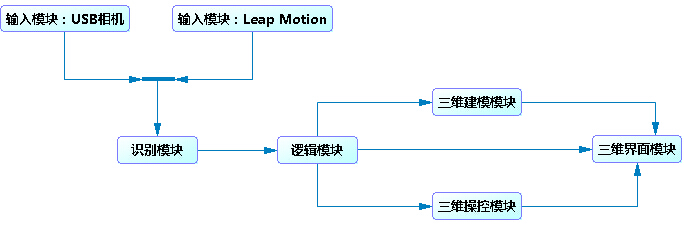
\includegraphics[width=0.8\textwidth]{chap2/system}
  \bicaption[fig:process]{系统概览图}{系统概览图}{Fig.}{system diagram}
\end{figure}

\section{系统介绍}
\subsection{系统概览}
本文系统着重研究混合现实眼镜下的交互界面、交互手段及空间设计应用中的具体设计,图\ref{fig:process}所示本文系统主要分为这几个模块:
输入模块、多通道识别模块、三维界面模块、逻辑模块、三维操控模块与建模模块。

%\begin{figure}[!htpb]
  %\centering
  %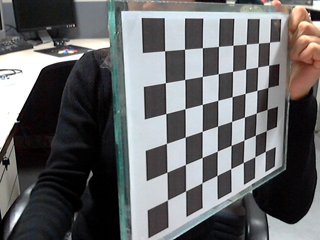
\includegraphics[width=0.24\textwidth]{chap2/camera_0_cap_1}
  %\hspace{1cm}
  %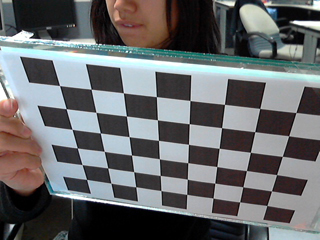
\includegraphics[width=0.24\textwidth]{chap2/camera_0_cap_2}
  %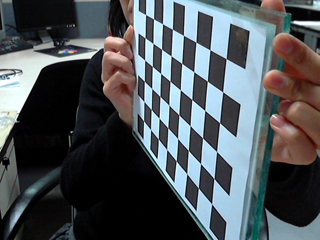
\includegraphics[width=0.24\textwidth]{chap2/camera_0_cap_12}
  %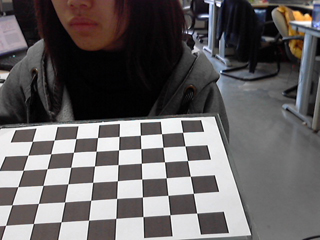
\includegraphics[width=0.24\textwidth]{chap2/camera_0_capture_1}
  %\bicaption[fig:chess]{棋盘格标定}{棋盘格标定}{Fig.}{Chessboard calibration}
%\end{figure}

\begin{figure}[!htpb]
	\centering
	\subfigure{\label{fig:chessboard:1}}\addtocounter{subfigure}{-2}
	\subfigure[Turn right]{\subfigure[向右偏转]
		{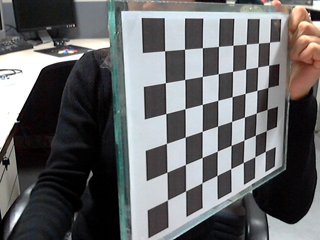
\includegraphics[width=0.22\textwidth]{chap2/camera_0_cap_1}}}		
	\subfigure{\label{fig:chessboard:2}}\addtocounter{subfigure}{-2}
	\subfigure[Turn down]{\subfigure[向下偏转]
		{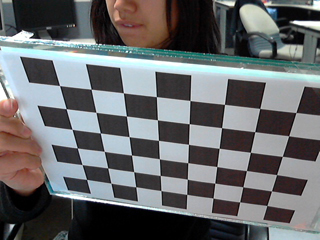
\includegraphics[width=0.22\textwidth]{chap2/camera_0_cap_2}}}		
	\subfigure{\label{fig:chessboard:3}}\addtocounter{subfigure}{-2}
	\subfigure[Turn left]{\subfigure[向左偏转]
		{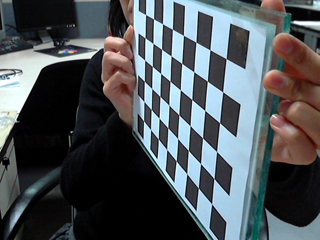
\includegraphics[width=0.22\textwidth]{chap2/camera_0_cap_12}}}	
	\subfigure{\label{fig:chessboard:4}}\addtocounter{subfigure}{-2}
	\subfigure[Turn up]{\subfigure[向上偏转]
		{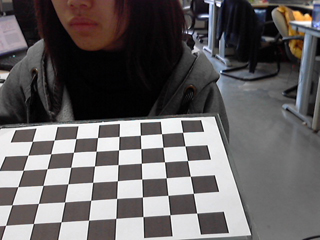
\includegraphics[width=0.22\textwidth]{chap2/camera_0_capture_1}}}		
	\bicaption[fig:chess]{棋盘格标定}{棋盘格标定}{Fig.}{Chessboard calibration}
	%\bicaption[总标签名]{}{中文总标题}{Fig.$\!$}{The total caption}
	\vspace{-1em}
\end{figure}

\subsection{输入与识别模块}
\label{sec:input}
	
本文系统在设计过程中涉及多种输入方式,本模块负责所有输入的标定。本文所设计的系统使用自制的混合现实眼镜ARGlasses作为系统输入,ARGlasses在演变过程中由不同硬件设备组成,输入部分有USB Camera, Leap Motion及改装过的广角USB Camera。 
为了模拟双目视觉的效果,系统之初采用两个横置USB Camera,
如图\ref{fig:chess}所示通过棋盘格进行独立标定,获得所需内参,图\ref{fig:chess}(a)、\ref{fig:chess}(b)、\ref{fig:chess}(c)和\ref{fig:chess}(d)分别是上下左右四个方向尽力偏转标定的演示,而后再进行双目标定。
图\ref{fig:stereoCalibration}显示通过双目标定后对原图像进行变换,变换前可从图\ref{fig:stereoCalibration}(a)中观察到左右二图的不匹配,而后左右眼图像(图\ref{fig:stereoCalibration}(c)})对齐效果更佳,可从背景的一些水平纹理中看到。
\begin{figure}[!htpb]
  \centering  
  \subfigure{\label{fig:stereoCalibration:before}}\addtocounter{subfigure}{-2}
	\subfigure[Left image before calibration]{\subfigure[标定前的左图]
		{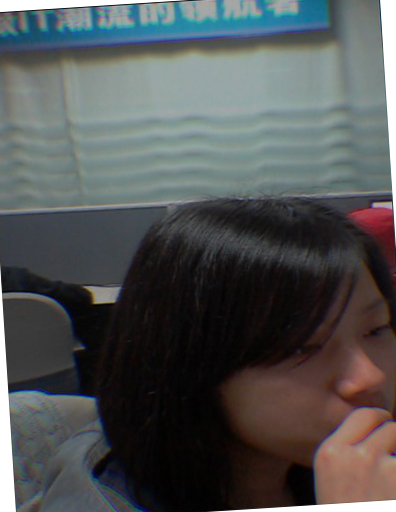
\includegraphics[width=0.225\textwidth]{chap2/beforeCalibration}}}		
	\subfigure{\label{fig:stereoCalibration:beforer}}\addtocounter{subfigure}{-2}
	\subfigure[Right image before calibration]{\subfigure[标定前的右图]
		{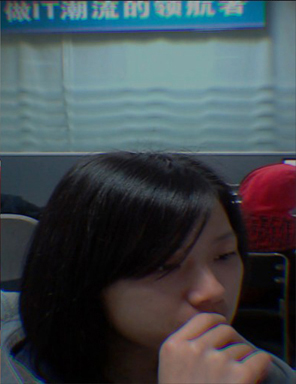
\includegraphics[width=0.225\textwidth]{chap2/afterCalibrationR}}}		
	\subfigure{\label{fig:chessboard:3}}\addtocounter{subfigure}{-2}
	\subfigure[Image after calibration]{\subfigure[标定后的图]
		{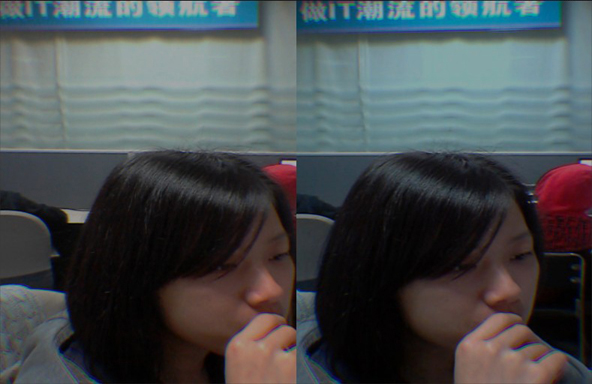
\includegraphics[width=0.45\textwidth]{chap2/afterCalibration}}}	
  \bicaption[fig:stereoCalibration]{双目标定}{双目标定}{Fig.}{stereo calibration}
\end{figure}
然后Leap Motion的采用是为了获得更稳定细致的手势信息,早期Leap Motion只提供具体的手部骨骼信息,为了将相机输入信息与Leap Motion的手部骨骼信息融合,系统自行设计了一套标定方法,系统通过在相同的位置呈现手势与棋盘格,获得多组对应数据进行点集映射得到粗略标定结果。
为了扩大捕捉到的场景视角,系统给相机增加了广角镜头,因此在输入处理过程中先对广角镜头捕获到的画面进行反扭曲处理,而后对反扭曲的结果进行棋盘格标定等操作,其效果可由图\ref{fig:WideLensUndist}可见。
棋盘格在图
\ref{fig:WideLensUndist}(a)中交叉线微微弯曲,而在图\ref{fig:WideLensUndist}(b)中反扭曲为直线,可见效果。

\begin{figure}[!htpb]
  \centering
  \subfigure{\label{fig:WideLensUndist:before}}\addtocounter{subfigure}{-2}
	\subfigure[Image before wide lens undistortion]{\subfigure[广角镜头反扭曲前的图]
		{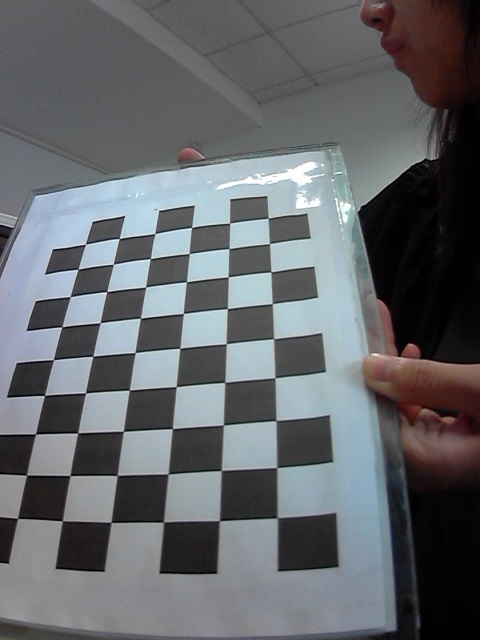
\includegraphics[width=0.3\textwidth]{chap2/camera_1_capture_6}}}		
	\subfigure{\label{fig:WideLensUndist:after}}\addtocounter{subfigure}{-2}
	\subfigure[Image after wide lens undistortion]{\subfigure[广角镜头反扭曲后的图]
		{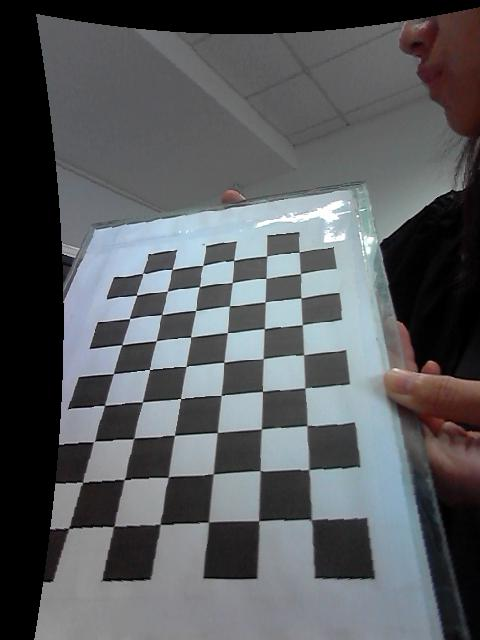
\includegraphics[width=0.3\textwidth]{chap2/undistcamera_1_capture_6}}}
  \bicaption[fig:WideLensUndist]{广角镜头反扭曲前后对比图}{广角镜头反扭曲前后对比图}{Fig.}{Undistortion of USB camera with wide lens}
\end{figure}

在研究的过程中,Leap Motion提供图像接口,可以获取拍摄所得源图像,于是系统结合Leap Motion所获取的源图像与相机图像进行匹配。
通过Leap Motion得到的原图进行反扭曲处理,由图\ref{fig:LeapMotionUndist}可见前后对比,棋盘格在图
\ref{fig:LeapMotionUndist}(a)中向右偏转,图\ref{fig:LeapMotionUndist}(b)中正面向前,图\ref{fig:LeapMotionUndist}(c)中向右偏转,然后将其作为混合现实眼镜的背景。
本模块最终输出标定过后的图像或手势信息,供识别模块进一步处理。
虽然输入模块相当重要,但并非本文重点所以之后并不再赘述。

\begin{figure}[!htpb]
  \centering
  \subfigure{\label{fig:LeapMotionUndist:left}}\addtocounter{subfigure}{-2}
	\subfigure[Turn right]{\subfigure[向右转]
		{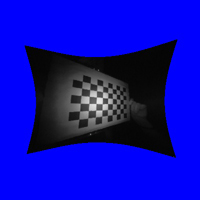
\includegraphics[width=0.3\textwidth]{chap2/undistort_399}}}		
	\subfigure{\label{fig:LeapMotionUndist:face}}\addtocounter{subfigure}{-2}
	\subfigure[Face to face]{\subfigure[正面]
		{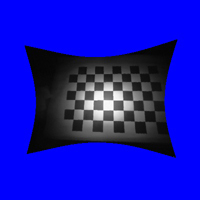
\includegraphics[width=0.3\textwidth]{chap2/undistort_299}}}		
	\subfigure{\label{fig:LeapMotionUndist:right}}\addtocounter{subfigure}{-2}
	\subfigure[Turn left]{\subfigure[向左转]
		{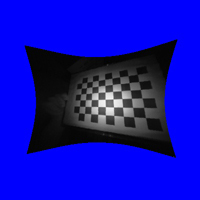
\includegraphics[width=0.3\textwidth]{chap2/undistort_219}}}
  \bicaption[fig:LeapMotionUndist]{Leap Motion反扭曲图}{Leap Motion反扭曲图}{Fig.}{Undistortion of Leap Motion images}
\end{figure}

识别模块主要有相机识别手势,Leap Motion识别手势,Oculus VR\upcite{Oculus}识别头部动作构成。
相机识别手势有以下几个步骤,首先获取原彩色图进行肤色提取,考虑到色彩空间在不同光线下并不稳定,所以这里设定了较广的肤色阈值,而后对超过手型大小阈值的肤色区域进行手型识别,根据形状判断是否含有手指,含有合法手指的区域便认定为是手型。标准的手型提取便是如此,之后根据手势的设计会有更细致的修改。
Leap Motion识别手势比较便捷,该设备官方提供手部骨架,可以直接分析其动作。
Oculus VR内置传感器,可以获得当前设备的角度,因而可以分析头部的动作信息,判断是否上仰。

\subsection{三维界面模块}
\label{sec:interface}
三维界面模块维护文所设计的系统界面,本文系统为混合现实眼镜设计了独有的三维界面,用来更好地配合用户的操作进行显示与交互。
三维界面由调色盘菜单和其他辅助信息组成,调色盘菜单地位等同桌面应用下的WIMP系列\upcite{Behr:2008:CND:1401132.1401164},负责让用户更直观地选择想要的命令。
其他辅助信息包括选中的立体包围盒,顶置提示板,骨骼小球都是本文所设计的系统运行中帮助用户更好地体验混合现实眼镜的可选配置,将在第\ref{chap:exp}章详细描述并评估。

\subsection{逻辑与操控模块}
\label{sec:logic}
逻辑模块负责连接识别结果与具体操作。结合识别到的手势,当前的环境,判断手势想表达的含义,比如在菜单出现时单手手指表示选择,而在物体被选中时表示单手操控。
据此调整三维界面上的显示,包括在顶置布告栏上更新状态,更改被选中的菜单样式进行提醒等。
逻辑模块还将输出具体指令下的操作参数,如旋转操作的轴参数与角度参数,传递给三维操控模块。

三维操控模块负责基本的平移旋转和缩放操控,通过输入的参数判断是哪种操控类型,然后根据参数进行实施操控,包括单手旋转和双手旋转时不一样的操控方式,也在该模块的处理之中。

\subsection{建模模块}
\label{sec:model}
建模模块针对三维建模用例,负责将用户的一系列建模指令转换成顶点。根据本文系统设计的自由虚拟网格平面,用户的输入全部转化为控制点,根据控制点该模块将绘制网格形成三维模型。
由于控制点的顺序随用户自定,所以该模块首先根据所有的控制点进行最优凸多面性估测用户绘制的形状,然后将不同层之间的控制点连接成三角面片。
除此之外在建模过程中自由虚拟网格平面的网格大小与方向都可由用户控制变换,针对被放缩与旋转的情况根据中心变换原则对所有控制点和网格平面进行点的相对位置的变换。在后文自由虚拟网格平面的具体设计中会详细描述。

\subsection{混合现实眼镜设备}
\label{chap:ARGlasses}

\subsubsection{混合现实眼镜初代}
\begin{figure}[!htp]
  \centering
  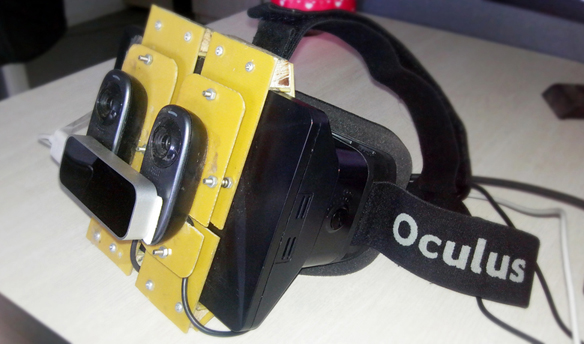
\includegraphics[width=0.6\textwidth]{chap2/ARGlassv1}
  \bicaption[fig:ARGlassesV1.0]{ARGlasses V1.0}{ARGlasses V1.0}{Fig.}{ARGlassesV1.0}
\end{figure}
图\ref{fig:ARGlassesV1.0}为混合现实眼镜的最初设计,由两个USB相机捕获彩色数据,放置在最前方,由Leap Motion捕获手指骨骼,安置在中间,然后通过自制的固定夹板将输入设备固定在Oculus VR上,用户可以通过Oculus VR看到输入设备捕获的现场从而达到视频透视。
在夹板上设有许多旋钮,可以简单调整相机的位置与角度,使两个相机互相间尽量保持一致的相对位置,且达到理想的标定误差。
初代设计的缺陷其一是质量太重,在实验过程中几乎所有参与者都在摘下眼镜后眼睛略感不适并反馈有点沉。
其二则是视野太窄,一个普通摄像头的水平视角在39°,垂直视角在31°,为了达到双目效果横置两个摄像头,于是每个眼睛的水平视角则为31°,与人眼本身接近平角的观察范围相差甚远,观察到的景象会有放大的感觉,让用户失去对深度的正确判断,故而第二个版本主要针对视角进行修改。

\subsubsection{混合现实眼镜广角版}
\begin{figure}[!htp]
  \centering
  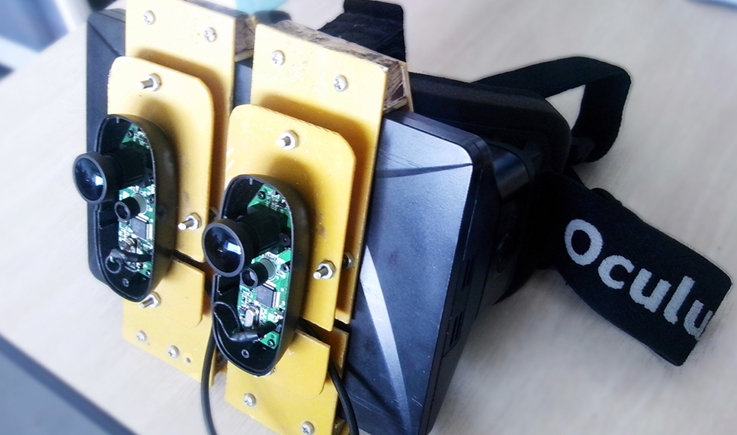
\includegraphics[width=0.6\textwidth]{chap2/ARGlassv2}
  \bicaption[fig:ARGlassesV2.0]{ARGlasses V2.0}{ARGlasses V2.0}{Fig.}{ARGlassesV2.0}
\end{figure}

图\ref{fig:ARGlassesV2.0}主要针对视角进行修改,可以看到原先的USB相机被拆到电路板层级并在摄像头元件前端安置了两个180°广角镜头,安装之后水平视角达到72°,虽然距离人眼的自然视角仍有距离,但比初代版本要宽广一些,并且质量上并没有很大变化。
但初代和广角版共同的缺陷在于双目相机之间的标定,双目标定可以做到对某一深度的物体进行匹配,从而左右眼可以合作观察该深度的物体,但是对于其他深度就会出现标定不合的情况,这是自制双目相机与视频透视融合的缺陷,也是接下来要解决的主要问题。

\begin{figure}[!htp]
  \centering
  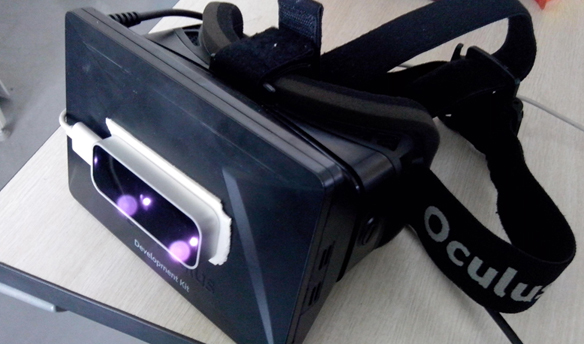
\includegraphics[width=0.6\textwidth]{chap2/ARGlassv3}
  \bicaption[fig:ARGlassesV3.0]{ARGlasses V3.0}{ARGlasses V3.0}{Fig.}{ARGlassesV3.0}
\end{figure}

\subsubsection{混合现实眼镜轻量级}

图\ref{fig:ARGlassesV3.0}则是最新版本,出于轻便性、视野及图像匹配的考虑,本文所设计的系统放弃彩色图像来源,直接使用Leap Motion作为唯一图像输入。
Leap Motion由于本身设备使用多角度的红外摄像头加灰阶Camera采集,可以捕捉到黑白景象,黑白灰阶随深度和热量而变。
其分辨率为640*240,虽然不高但和显示设备Oculus VR的800*600也相去不远。
\begin{table}[!hptb]\renewcommand{\arraystretch}{1.2}
  \centering
  \bicaption[table:arglass]{本文工作所制作的三代混合现实眼镜对比}{本文工作所制作的三代混合现实眼镜对比}{Table}{Comparison among three generations of Mixed Reality Glasses in this work}
  \begin{tabular}{*{4}{L{.32\textwidth}}} \toprule
  %\begin{tabular}{@{}ccc@{}} \toprule
    眼镜名称 & 优点 & 缺点 \\
	\midrule
    混合现实眼镜初代 	& 		1.彩色图像 		& 	\hspace{150pt}1.笨重\hspace{90pt}2.视野狭窄\hspace{90pt}3.存在设备间标定误差\\	
	%&&2.视野狭窄\\
	%&&3.存在设备间的标定误差\\
	%\vspace{1em}
    混合现实眼镜广角版 & 1.彩色图像\hspace{80pt}2.视野有扩大\vspace{1em}& 1.仍显笨重\hspace{90pt}2.存在设备间标定误差\\
	%&2.视野有扩大 &2.存在设备间的标定误差	\\
	%\vspace{1em}
    混合现实眼镜轻量级 & 1.视野符合人眼\hspace{100pt}2.轻巧\hspace{100pt}3.单一输入设备无标定误差& 1.灰色图像 \\
	%&2.轻巧 &\\
	%&3.单一输入设备无标定误差&\\
	\bottomrule
  \end{tabular}
\end{table}
关键其一他的视角到达110°以上,戴上之后和直接视物差距不大,其二由于是将一个完整的场景分割为左右眼两幅图像传递给用户,于是并没有两幅图像间不匹配的困扰,同时由于少了USB相机和固定用的夹板,整个设备一下子轻了很多。
最终三维界面与操控的设计基于混合现实眼镜初代,而三维建模应用的设计基于混合现实眼镜轻量级实现。

\section{本章小结}
本章概要地描述了本文系统的研究方法,然后介绍了本文系统的流程与模块划分,通过本章可以直观明朗地了解到本文系统的输入输出与用例,方便在对其中细节更深的探索前有一个完整的概念。
然后介绍了本文所设计的系统依赖的硬件设备:自制的混合现实眼镜,讲述其构造与发展历程,三代混合现实眼镜的比较可见表\ref{table:arglass}。
本文系统都构建在该设备之上,虽然硬件制作不是本文的重点,但其准确率、精度与轻便性对本文所设计的系统的实验评估都有很大影响,在此处特别介绍下。
